\makeatletter
\def\input@path{{../}}
\makeatother

\documentclass[/main.tex]{subfiles}
\graphicspath{{./pics/}{ch5/pics/}}
\begin{document}

\onlyinsubfile{\textpages}
\chapter{Double Beta Decay to Excited States Results}
Now that we have found and characterized a specific detection signature for each decay mode, we can apply this search to data.
This result will look at open runs from datasets 1~through 6a that were designated silver or gold in run quality.
The duty cycle and changes that define each data set are shown in figure~\ref{fig:dutycycle}.
These were taken from January 12, 2016 to April 18, 2018, and contains a total of 13.4~kg~y of isotopic exposure for module~1 and 7.9~kg~y for module~2.
Approximately half the data in these datasets is blinded, and is not included in this analysis.
The \MJD\ uses a statistical blinding scheme in which 3/4 of runs are blinded administratively (i.e. through file access) in cycles of 31~hrs of unblinded runs followed by 93~hrs of blinded runs.
The data is unblinded in a staged fashion, where first single-site events, not including any interesting physics regions are unblinded (i.e. no background ROI, \znbb\ to the ground state ROI, low energy or multisite data).
This data is used for a variety of data validation checks prior to unblinding of any other data.
The remaining data are separately unblinded after a collaboration review for individual analyses and users.
For this analysis, the multi-site data has been left blinded.
\\
\begin{figure}[h]
  \centering
  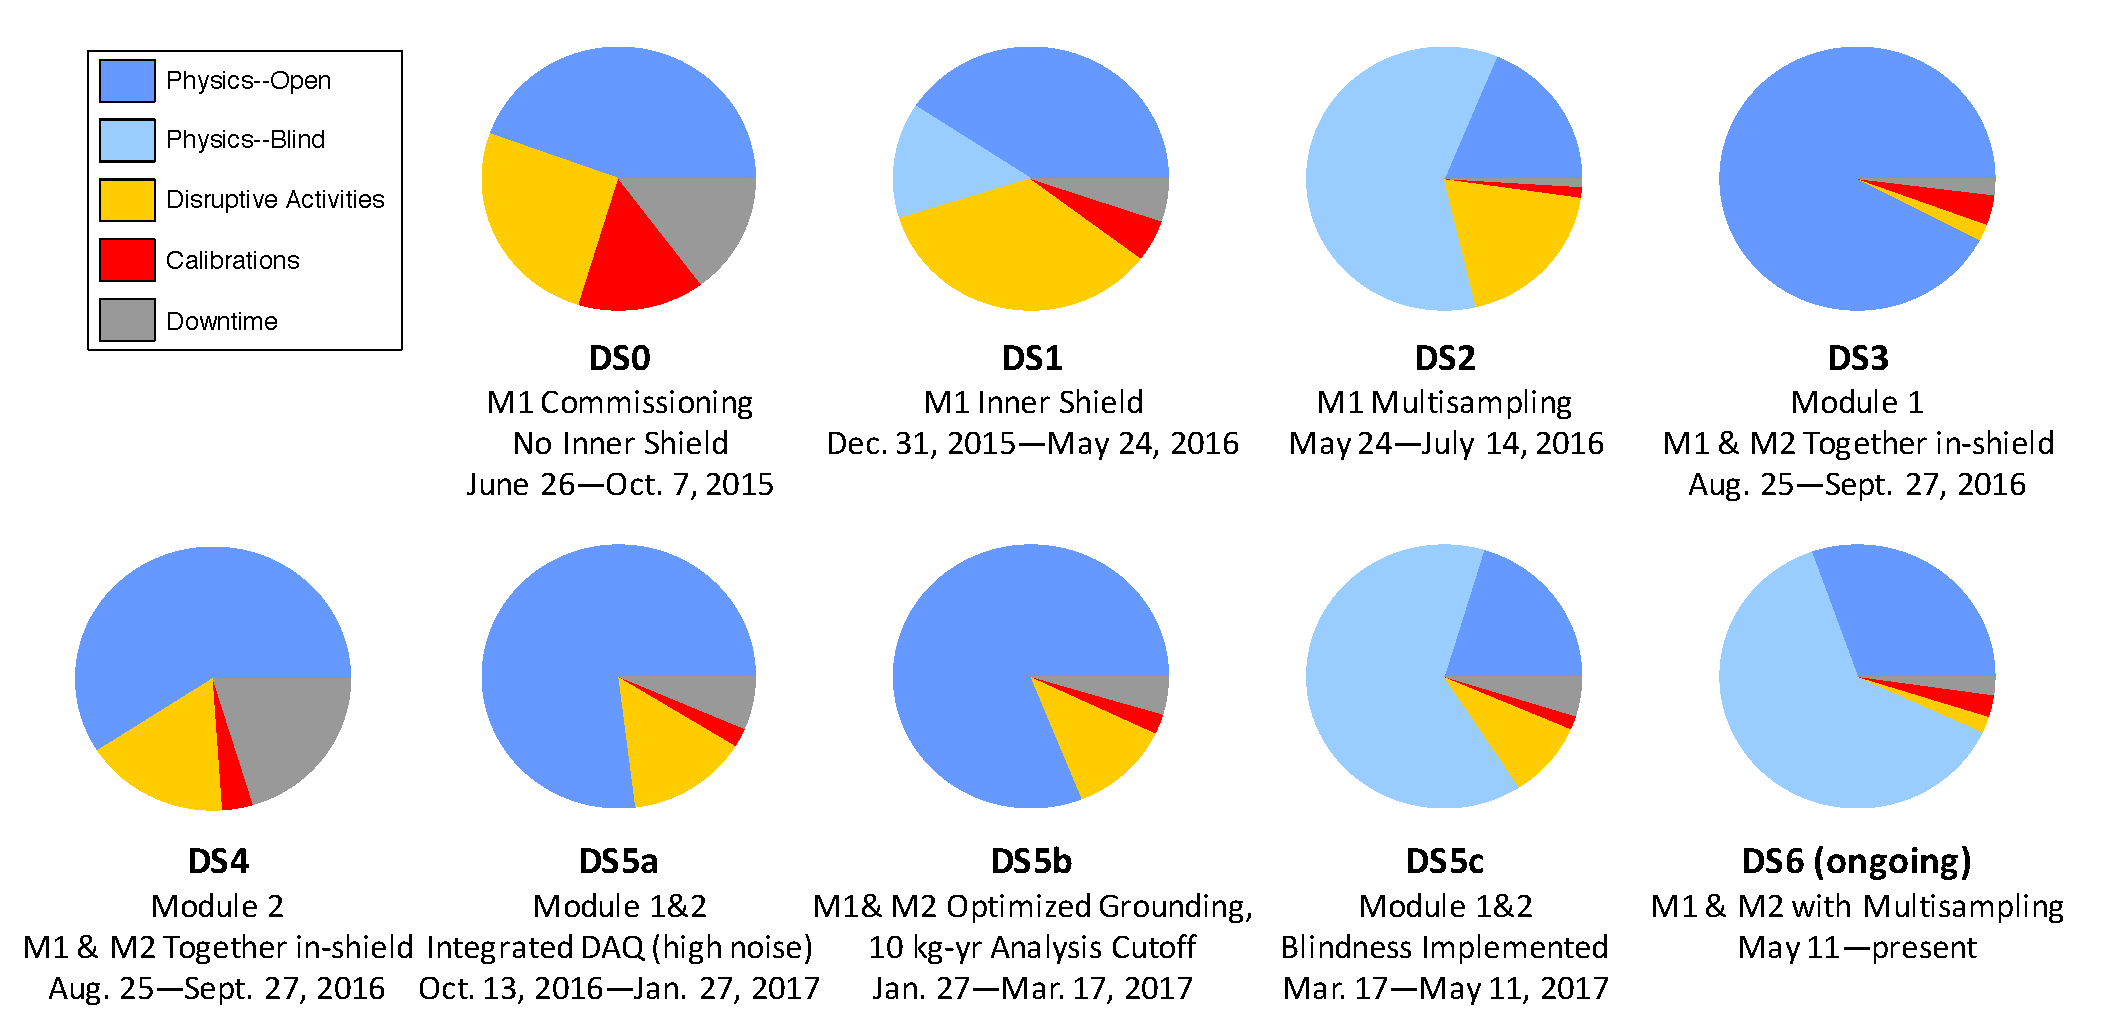
\includegraphics[width=0.9\linewidth]{dutycycle}
  \caption[Dataset and Duty Cycle Summary]{\label{fig:dutycycle}
    The duty cycles for each major dataset, and a brief discription of the major changes in configuration that define each data set.
  }
\end{figure}

In the open multi-site data, 5558 multi-detector events were observed.
A histogram of the event multiplicities is shown in figure~\ref{fig:datamult}, and a spectrum of all multiplicity~2 event energies is shown in fiture~\ref{fig:data2D}.
\begin{figure}[h]
  \centering
  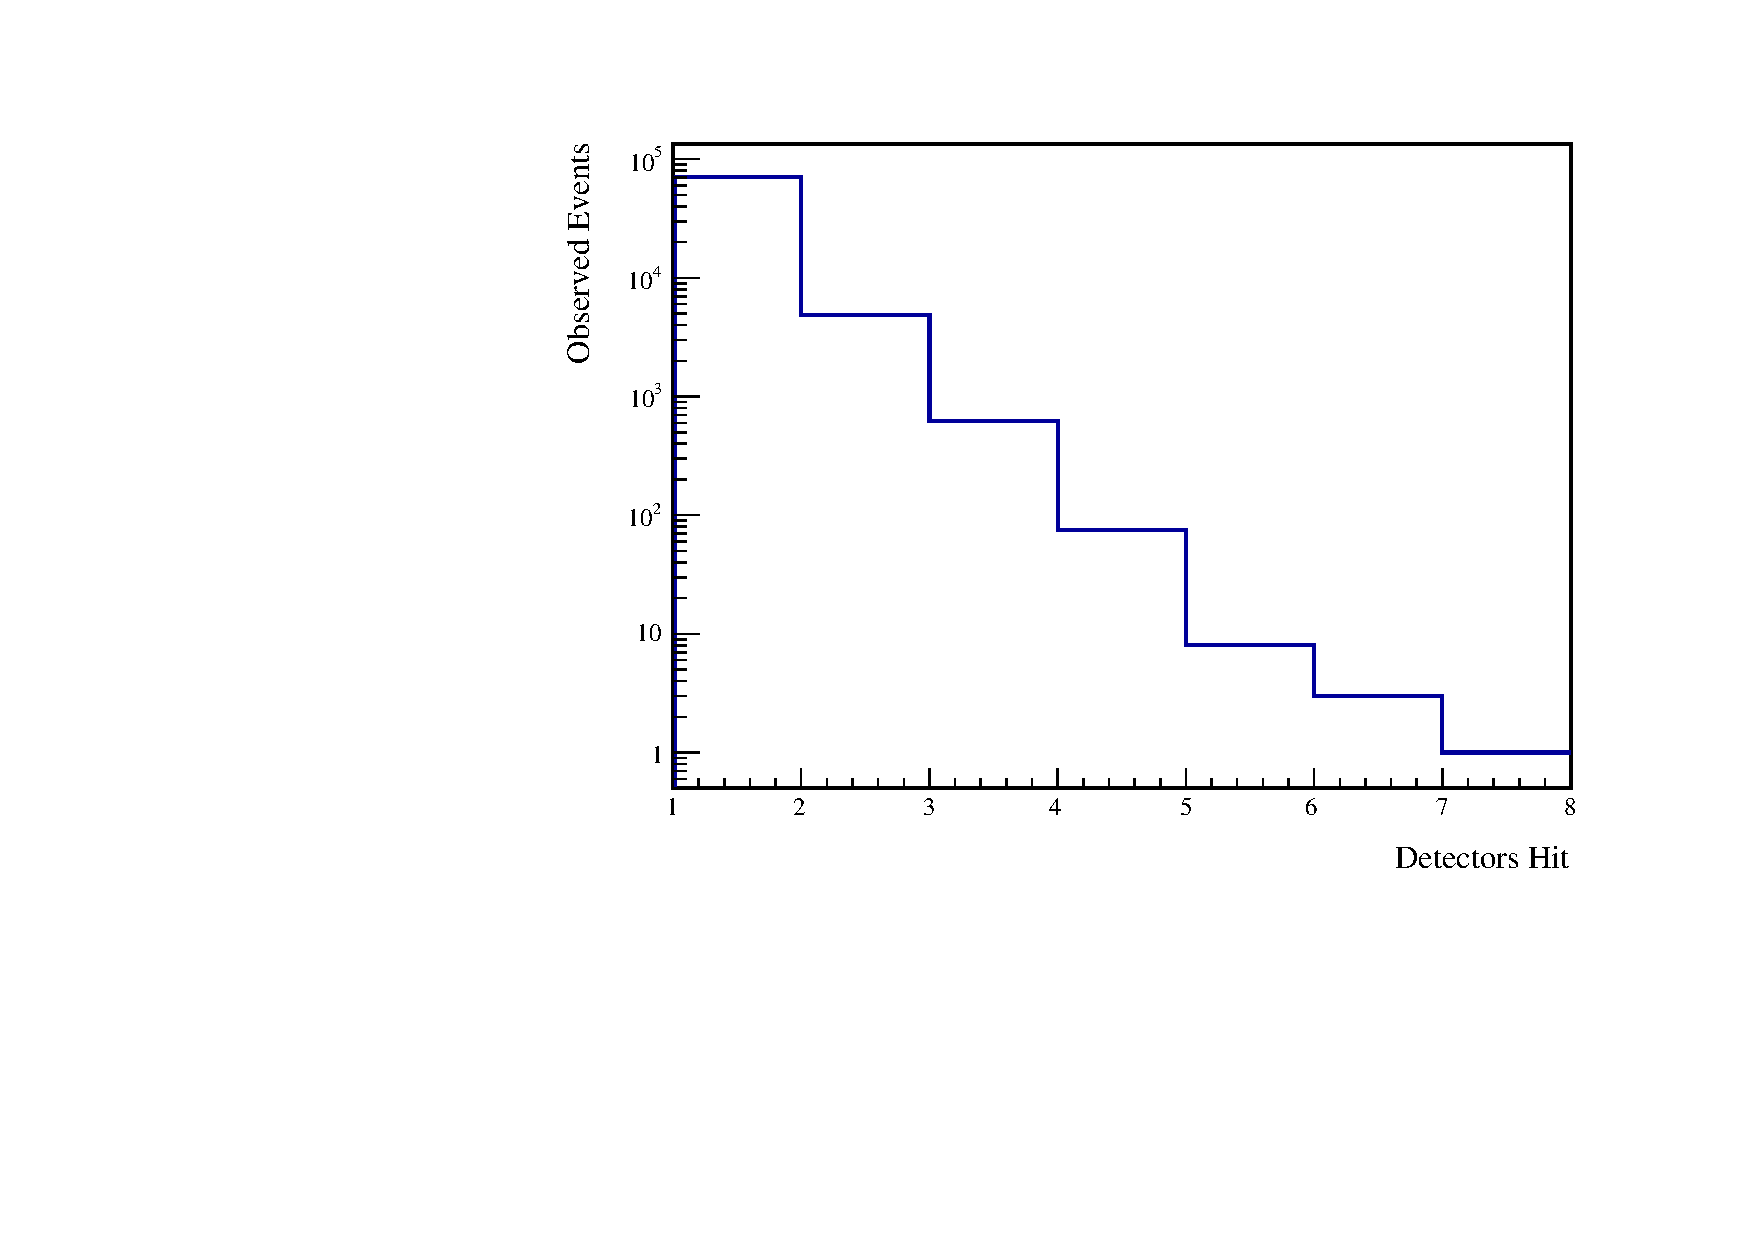
\includegraphics[width=.6\linewidth]{DataMultiplicity}
  \caption[Measured event multiplicities]{\label{fig:datamult}
    The measured multiplicities for events in datasets~1-6a. For multiplicity~1 events, only events with energy between 40~keV and 4~MeV were considered.
  }
\end{figure}
\begin{figure}[h]
  \centering
  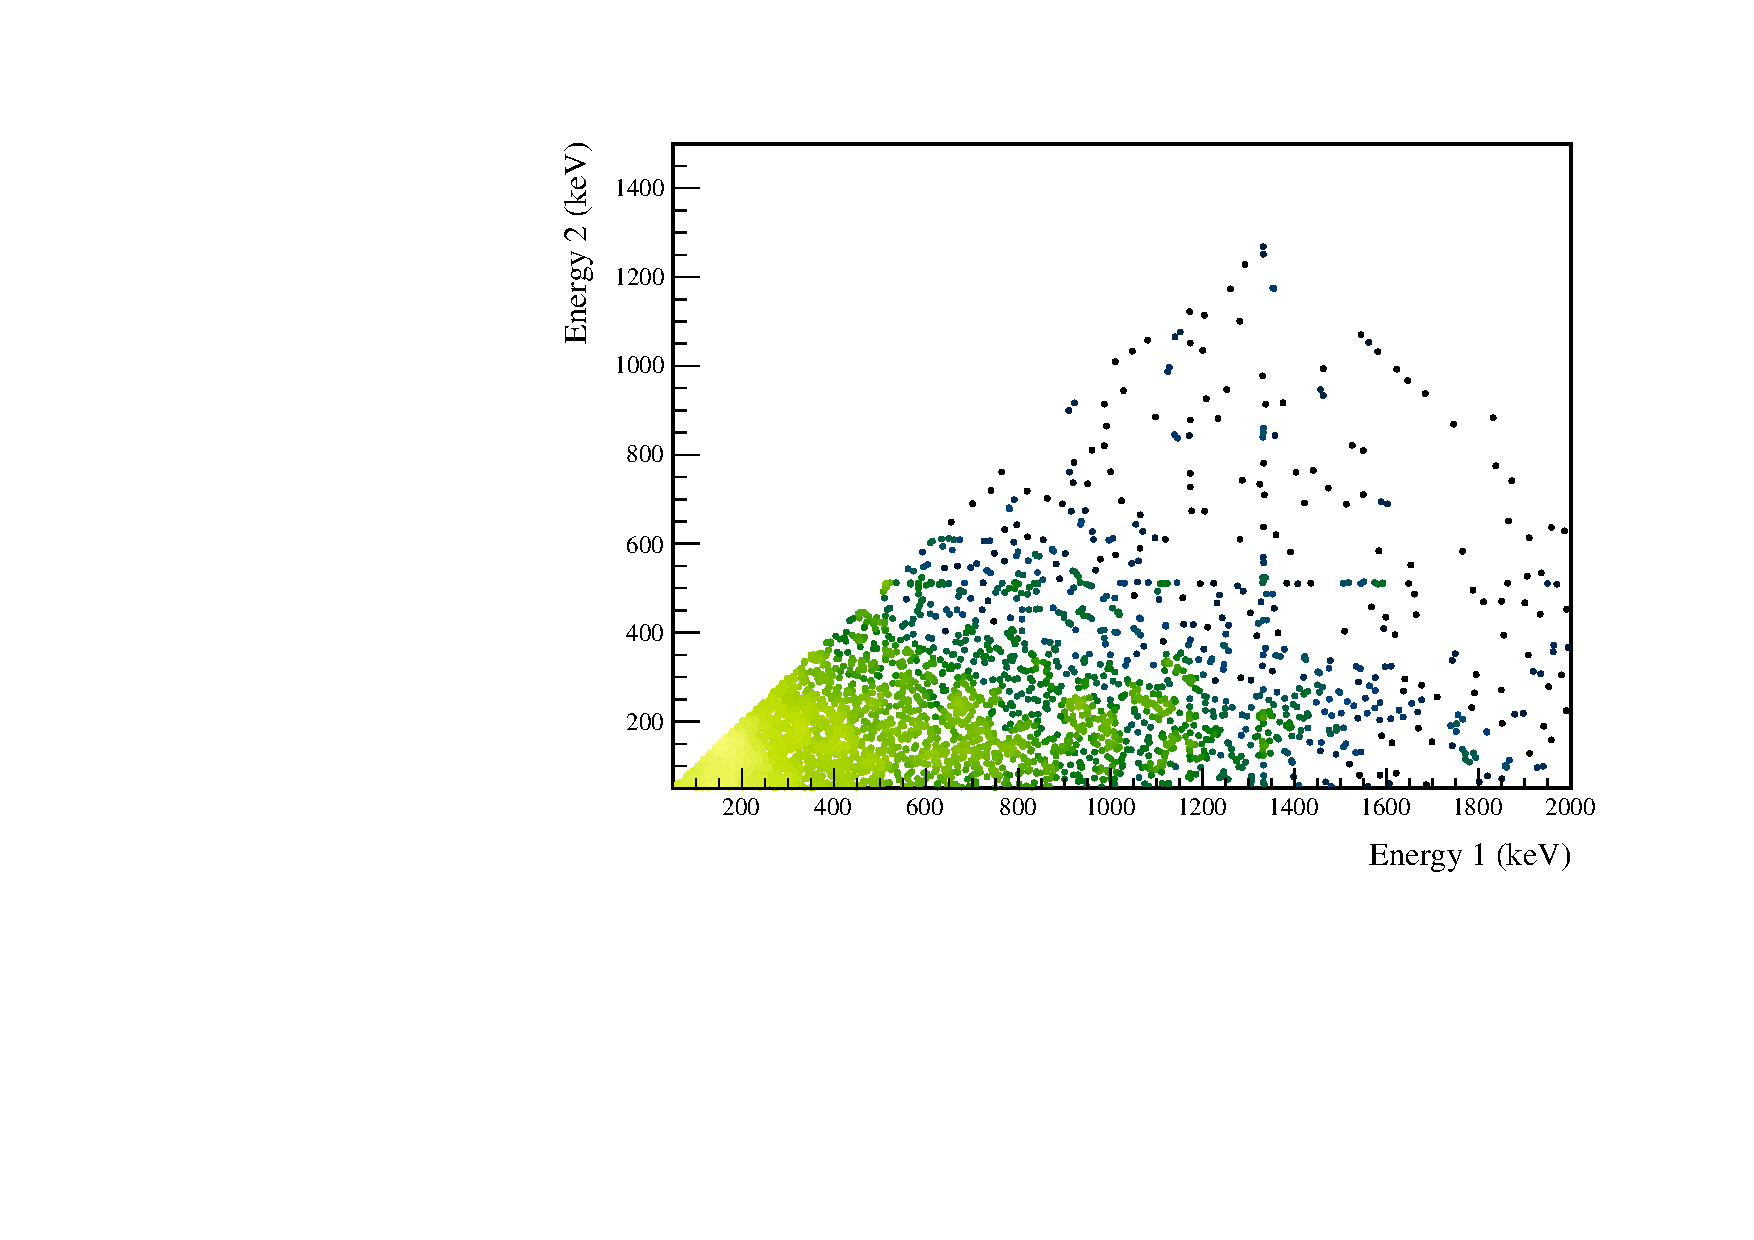
\includegraphics[width=.8\linewidth]{Data2D}
  \caption[Measured energy spectrum of multiplicity~2 events]{\label{fig:data2D}
    Measured energy spectrum of multiplicity~2 events in datasets~1-6a.
  }
\end{figure}

\section{Validation}
In addition to the basic run selection and data cleaning validation checks that are run on all multiplicity~1 data, we will perform some additional checks on high multiplicity data.
As previously, this section will describe these checks applied to the \tnbb\ to the \SP{0}{+}{1} state of \Se{76}.
Similar checks are performed on other decay modes in appendix~\ref{app:allresults}.

\subsection{Data Rate}
Any spikes in the rate of multisite events would potentially indicate problems with run selection or data cleaning.
Significant variation in the data rate is expected due to changes in which detectors are active.
For this reason, the rate of multisite events with respect to the effective exposure, which is the exposure times the detection efficiency of \bbes\ events is used instead.
This quantity is interesting because the rate of observed \bbes\ events should be constant wtih respect to it.
The changes in detection efficiency from one subdataset to another for both backgrounds and \bbes\ are highly correlated and driven by which detectors are enabled.
For this reason, we can reasonably expect that the backgrounds should also have a nearly constant rate with respect to effective exposure, although differences between background source positions and the distribution of \Ge{76} in the detectors imply that some differense should be expected.
Figure~\ref{fig:eventrate} indeed shows a slow reduction in the overall background rate over time.
One possible explanation for this is that a significant quantity of \Ge{68} exists in natural HPGe detectors as a result of cosmogenic activation, and has a half-life of 271~days, which is observable on the timescale of the \MJD's operation.
\iso{68}{Ga} is a $\beta^+$ emitter which is a part of the \Ge{68} decay chain, which produces two 511~keV $\gamma$s, resulting in many \msmd events.
\begin{figure}[ht]
  \centering
  \subfloat[Module 1]{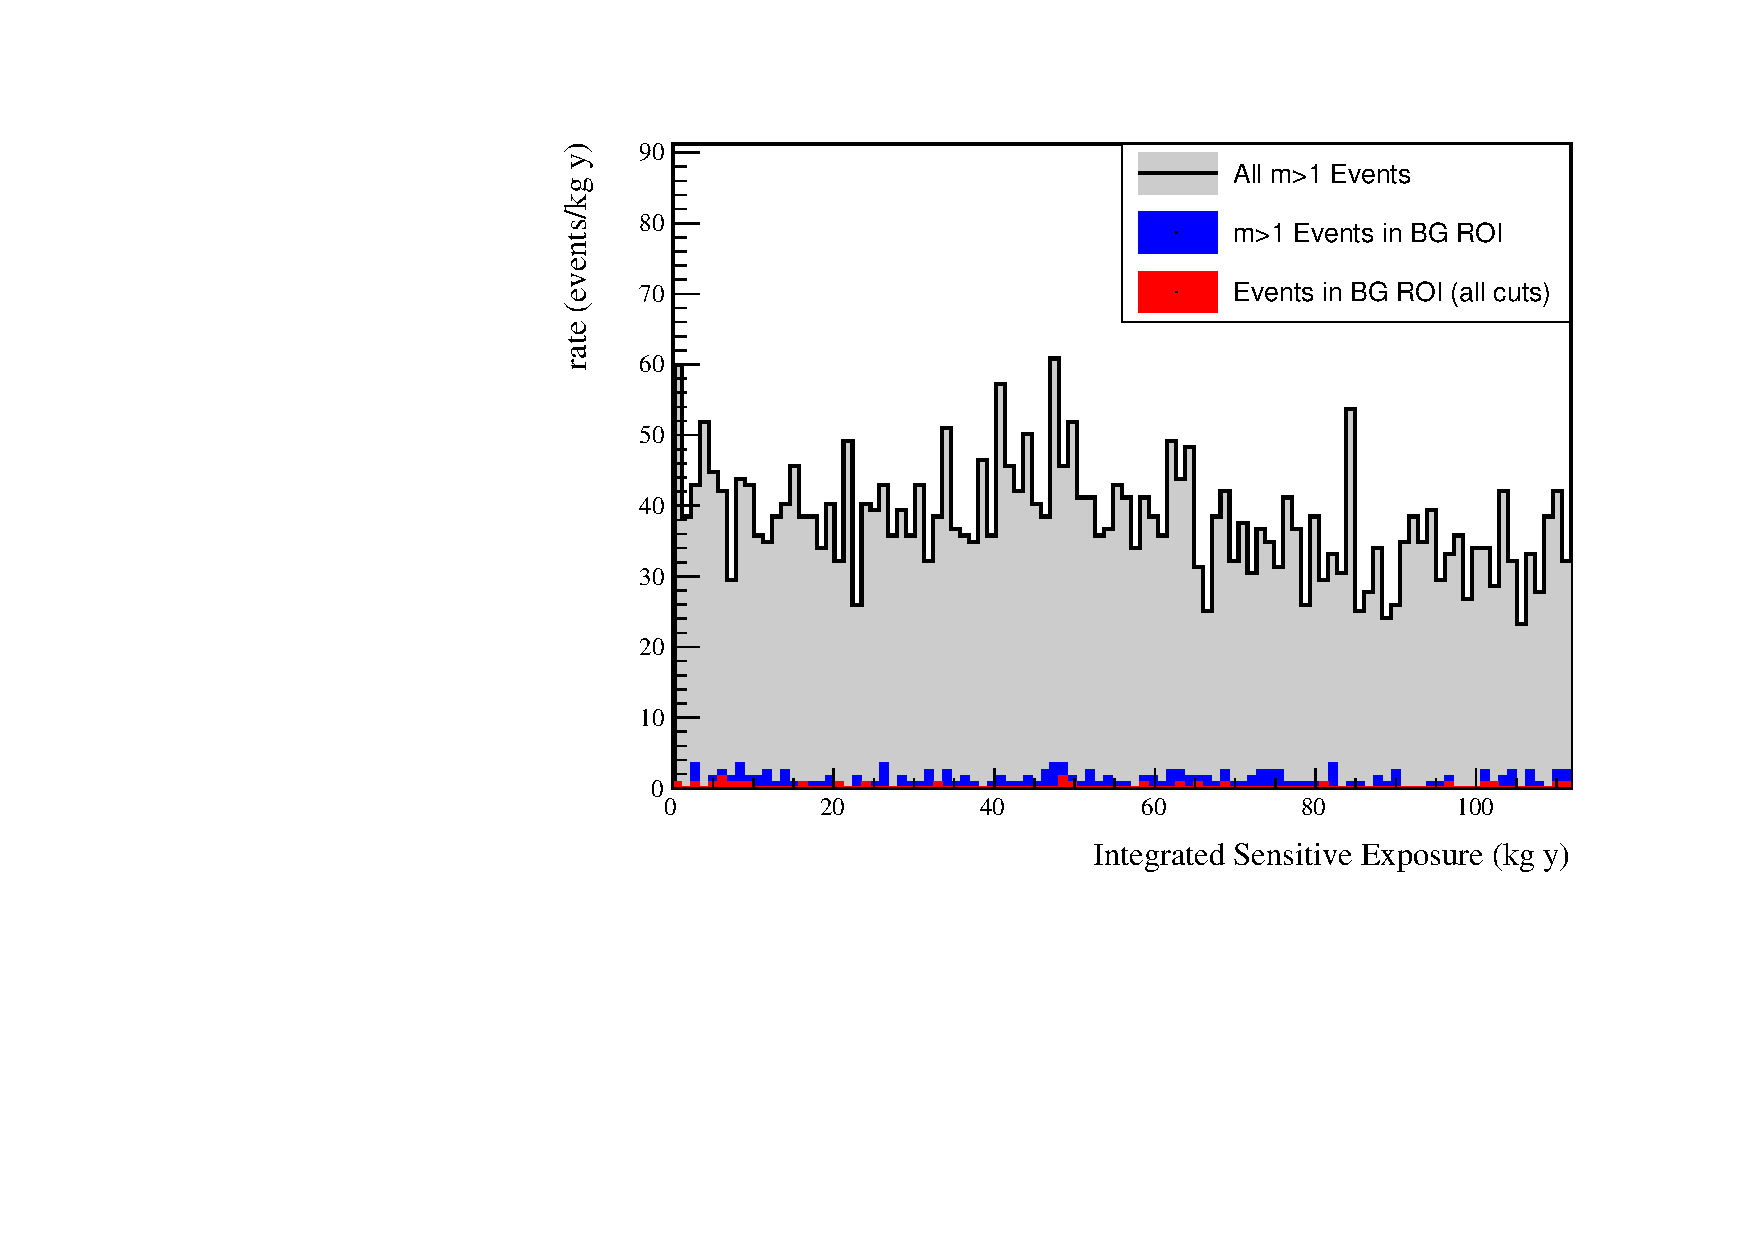
\includegraphics[width=.5\linewidth]{M1datarate}}
  \subfloat[Module 2]{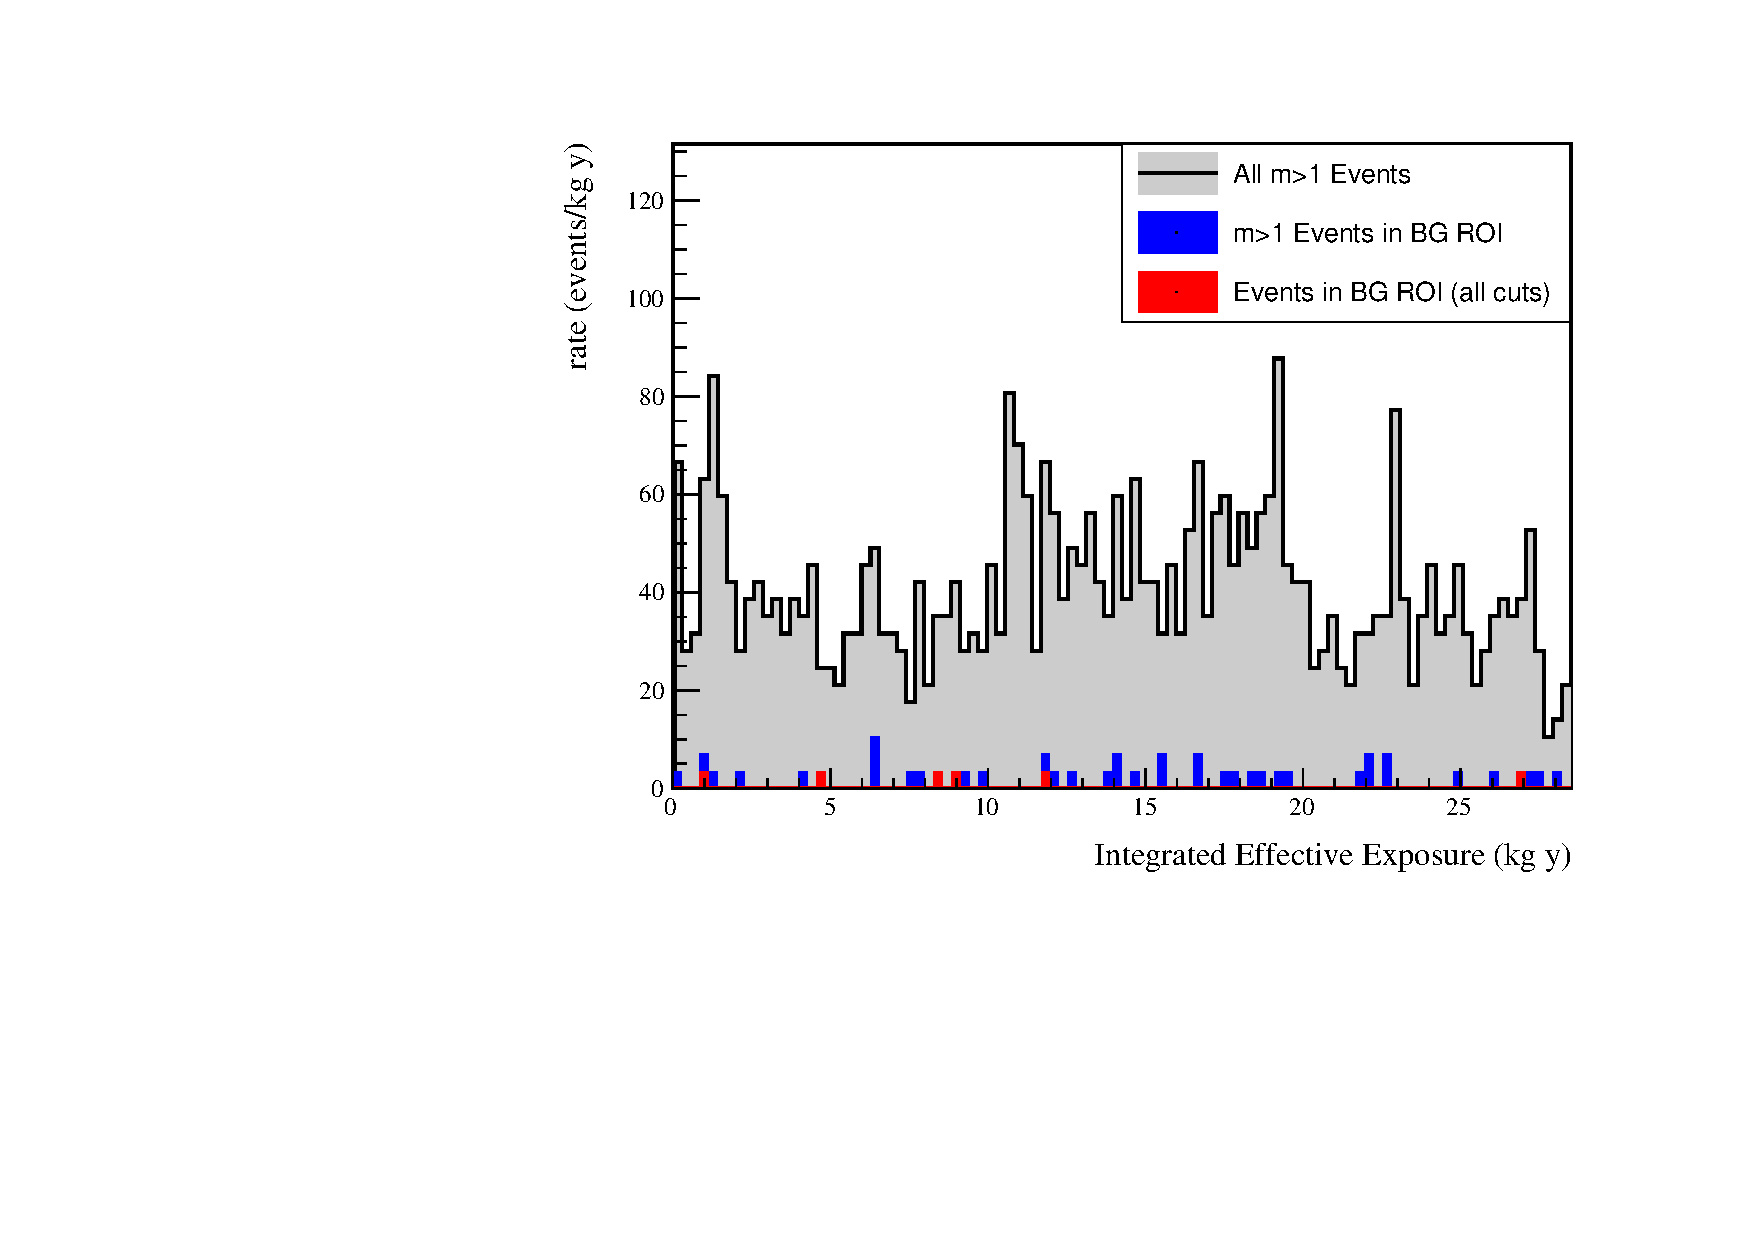
\includegraphics[width=.5\linewidth]{M2datarate}}
  \caption[Event rate in both modules with respect to effective exposure]{\label{fig:eventrate}
    Event rate with respect to effective exposure, or the detection efficiency of the \tnbb\ decay to the \SP{0}{+}{1} excited state times the exposure. Integrated exposure is the total effective exposure prior to an event. The background rate is expected to be mostly flat.
  }
\end{figure}


\subsection{Background Cut Evaluation}
A second important check to ensure that the cuts applied to each \bbes\ mode is to compare each cut efficiency to the expected background cut efficiency.
Since the background model used for this analysis uses preliminary results, disagreement between the expected and measured cut efficiencies could indicate a difference between the background model and the measured backgrounds rather than a problem with the application of cuts.
However, any major discrepencies could indicate a bug in the analysis.
To perform this comparison, the cut efficiencies are measured both in terms of the total number of events cut, $\epsilon_{total}$ and the number of events that are uniquely cut, $\epsilon_{unique}$ (i.e., not cut by any of the others).
Table~\ref{tab:bgcutstable} lists each cut for the \bbes\ decay to the \SP{0}{+}{1} state and the expected and measured cut efficiencies.
The expected background cut efficiencies, $\langle\epsilon\rangle$ represent the fraction of events cut, averaged over all datasets, weighted by exposure.
The measured background cut efficiencies, $\hat{\epsilon}$ represent the measured fraction of events cut.
Statistical uncertainties in the expected efficiencies are neglible compared to the uncertainties in the measured efficiencies, and are not included.
The sacrifice is the number of events uniquely sacrificed by the cut.
$\Delta \mathrm{DP}$ is the expected improvement in discovery potential, as defined in appendix~\ref{app:sens} as a result in the cut.
Figure~\ref{fig:datacuts2D} shows the effects of data cuts on multiplicity~2 events.
Figure~\ref{fig:cutsroi} shows the effects of cuts on events in the ROI in both measured and simulated data.

\begin{figure}
  \centering
  \includegraphics[width=0.8\linewidth]{Data2Dcuts}
  \caption[Effect of data cuts on measured multiplicity 2 events]{\label{fig:datacuts2D}
    Energy spectrum of multiplicity~2 events. Red events are events that are cut. For blue events, at least one of the hits passes all cuts; however, the other hit may fail. For green events, one of the hits must both pass all cuts and place the event in the BG or ES ROI.
  }
\end{figure}

\begin{figure}
  \centering
  \subfloat[Measured ROI Events]{\includegraphics[width=0.5\linewidth]{DataAllCuts}}
  \subfloat[Simulated ROI Events]{\includegraphics[width=0.5\linewidth]{BGAllCuts}}
  \caption[Effect of data cuts on ROI events in measured and simulated data]{\label{fig:cutsroi}
    Effect of cuts on all events in the BG and ES ROIs. Events are applied in sequence from top to bottom, meaning that if an event is cut by multiple cuts, it will be colored based on the first cut that applied. Both the simulated and measured event spectra are shown for comparison.
  }
\end{figure}

\begin{sidewaystable}[p]
  \centering
  ../../appAllResults/tables/table_2vBB_ES0_1_bgcuts.tex
  \caption[Detection efficiency summary for \tnbb\ to the \SP{0}{+}{1} state of \Se{76}]{\label{tab:bgcutstable}
    Table of detection efficiencies and uncertainties for \tnbb\ of \Ge{76} to the \SP{0}{+}{1} state of \Se{76}.
  }
\end{sidewaystable}

\section{Results}


\subsection{Statistical Methods}
Neyman confidence intervals are computed for each peak in each \bbes\ decay mode, and each module.
For a given peak $k$, the expected number of signal counts is
\begin{equation}
  \langle s_k\rangle = \ln2 \frac{N_A}{m_{76}}\epsilon_k\frac{M_{iso}T_{live}}{T_{1/2}}
\end{equation}
where $M_{iso}$ is the total isotopic mass and $T_{live}$ is the livetime ($M_{iso}T_{live}$ is the exposure and is calculated in section~\ref{sec:subdatasets} to be $13.356\pm0.021$ for module~1 and $7.872\pm0.13$ for module~2.
$\epsilon_k$ is the total detection efficiency of the decay mode using peak $k$, and is calculated in chapter~\ref{ch:4}, and can be found in appendix~\ref{app:allresults}.
$m_{76}=0.0759214$~kg is the molar mass of \Ge{76}, and $N_A=6.02214076\times10^{23}$ is Avagadro's number.
Fun fact: an Avagadro's number of avocados has approximately the volume of Mars.
We will define the single count half-life to be
\begin{equation}
  T^*_k=\ln2 \frac{N_A}{m_{76}}\epsilon_kM_{iso}T_{live}
\end{equation}
which is the decay half-life that would produce on average one count in signal ROI $k$.
\\
Because of the nearly background free nature of this search, a likelihood construction is used that assumes Poisson statistics for the number of counts in the signal and background ROIs.
\begin{equation}
  \label{eq:rolke}
  \begin{aligned}
    \mathcal{L}(T_{1/2},T^*_k,b_k|n_k,m_k,\langle T^*_k\rangle, \sigma_{T^*,k},\tau)
    &=\frac{\mu_k^{n_k}e^{-\mu_k}}{n_k!} \cdot \frac{(b_k\tau)^{m_k}e^{-b_k/\tau}}{m_k!} \cdot
    \frac{1}{\sigma_{T^*,k}\sqrt{2\pi}}e^{-\frac{(T^*_k-\langle T^*_k\rangle)^2}{2\sigma_{T^*,k}^2}} \\
    \mu_k &= s_k+b_k = \frac{T^*_k}{T_{1/2}} + b_k
  \end{aligned}
\end{equation}
$T_{1/2}$ represents the decay mode half-life and is the parameter of interest.
$T^*_k$ and $b_k$ are nuisance parameters representing the measured single count halflife and expected backgrounds in the ES ROI, respectively.
$\mu_k$ is the total expected number of counts, combining background and signal, in the ES ROI.
$n_k$ is the measured number of events in the ES ROI and is expected to be drawn from a Poisson distribution with mean $\mu_k$.
$m_k$ is the measured number of events in the BG ROI and is expected to be drawn from a Poisson distribution with mean $b_k/\tau$, where $\tau$ is the ratio between the number of expected background counts in the BG ROI to the number in the ES ROI.
Note that since these events are \msmd, it is possible for multiple hits in the event to fall into one of the ROIs; however, we will choose a single hit to represent the whole event.
In this case, any hit that falls into the ES ROI takes precedence over any hit that falls into the BG ROI, and if multiple hits fall into the ES ROI, one is chosen at random.
$\tau$ is usually determined based on the background simulation; however, in cases where the simulation statistics are limited after applying all cuts, a flat background is assumed and the ratio of the ES ROI width to the BG ROI width is used.
$\langle T^*_k\rangle$ represents the expected value of $T^*_k$ based on previous measurements of exposure and detection efficiency, which is assumed to have Gaussian uncertainty:
\begin{equation}
  \sigma_{T^*,k} = \langle T^*_k\rangle\sqrt{(\frac{\sigma_{\epsilon,k}}{\epsilon_k })^2 + (\frac{\sigma_{exposure}}{M_{iso}T_{live} })^2}
\end{equation}
The implementation of equation~\ref{eq:rolke} is performed by the \texttt{TRolke} class in ROOT \cite{2005rolke}.
This likelihood function is used to compute a likelihood ratio
\begin{equation}
  \mathrm{LR}(T_{1/2}) = \frac{\mathrm{sup}_{T^*_k,b_k}(\mathcal{L}(T_{1/2},T^*_k,b_k|n_k,m_k,\langle T^*_k\rangle, \sigma_{T^*,k},\tau))}{\mathrm{sup}_{T_{1/2},T^*_k,b_k}(\mathcal{L}(T_{1/2},T^*_k,b_k|n_k,m_k,\langle T^*_k\rangle, \sigma_{T^*,k},\tau))}
\end{equation}
The \texttt{TRolke} class analytically computes the supremum over $T^*_k$ and $b_k$, returning the log-likelihood difference.
$T_{1/2}$ is restricted to positive values.
Since the likelihood ratio is expected to be $\chi^2$-distributed, to construct a 90\% confidence interval, we seek the values of $T_{1/2}$ corresponding to a log-likelihood ratio value of 2.7.
In cases where the lower limit is found to be $<0$, a lower limit on the half-life is reported.
\\
After constructing confidence intervals for each peak and module individually, a combined confidence interval is constructed for each \bbes\ decay mode.
A combined log-likelihood over all peak/module combinations $k$ is defined by
\begin{equation}
  \mathcal{L}(T_{1/2}) = \sum_{k=0}^{N} \mathrm{sup}_{T^*_k,b_k}(\mathrm{log}(\mathcal{L}(T_{1/2},T^*_k,b_k|n_k,m_k,\langle T^*_k\rangle, \sigma_{T^*,k},\tau)))
\end{equation}
This construction relies on the fact that the $T^*_k$ and $b_k$ values across each peak can be independantly maximized, enabling the continued use of the \texttt{TRolke} implementation.
A combined likelihood ratio is constructed and used to compute a confidence interval as above.
Table~\ref{tab:alllimits} contains the limits constructed for each decay mode, peak and module.
For all modes, a lower half-life limit is set.
\\
Note that each decay mode is analyzed independantly.
The problem with this approach is that all decay modes have the 559~keV peak in common, meaning that the results will be correlated.
For this result, since all modes only have a lower limit on half-life set, this approach is not problematic since for any individual mode, we would take the supremum over all other half-lives, which would be at or near infinity, resulting in the same sets of equations used here.
However, if the \bbes\ to the \SP{0}{+}{1} mode is discovered, it will become necessary to perform a full combined analysis.
\\
The detection sensitivity is computed by constructing a toy Monte Carlo for each decay mode, assuming that each $T_{1/2}$ is infinite.
For each sample $i$, a random $n_i$ and $m_i$ is drawn from a Poisson distribution with mean $n_k$ and $m_k$.
The confidence interval for a measurement with these values is computed.
The median sensitivity is extracted by taking the median lower half-life limit over all samples.
For the results in table~\ref{tab:alllimits}, 100001 samples were used.
\\
\subsection{Limits and Sensitivities}
\begin{figure}[h]
  \centering
  \includegraphics[width=.8\linewidth]{DataROIs}
  \caption[Measured events after all cuts with ROIs drawn]{\label{fig:roievents}
    Events that pass all cuts for the \tnbb\ to \SP{0}{+}{1} decay mode. The ES and BG ROIs are highlighted. Note that these ROIs undergo small variations from dataset to dataset, and the ROIs drawn here are averaged over all datasets. The energies shown in this spectrum are the energies of the hit that places the event in the ROI. A single event will only be placed once into an ROI; however, as drawn here, if multiple hits in a single event fall into an ROI, they will all be drawn.
  }
\end{figure}
The limits and sensitivities for each peak and module individually, and the combination for each mode, are shown in table~\ref{tab:alllimits}.
Figure~\ref{fig:roievents} shows the event spectrum after all cuts have been applied with both ROIs highlighed.

\begin{table}[h]
  \footnotesize
  \centering
  \begin{tabular}{|c|c|c c c c c|c|c|}
\hline  Decay Mode & Peak & Module & $n_{ROI}$ & $m_{BG}$ & \makecell{Expected\\ROI BGs} & $T^*\,(\times 10^{23} \mathrm{y})$ & \makecell{$T_{1/2}\,(\times 10^{23} \mathrm{y})$ \\ 90\% Limit} & \makecell{$T_{1/2}\,(\times 10^{23} \mathrm{y})$ \\ 90\% Sensitivity} \\
\hline
\multirow{5}{*}{\decaySP{2}{0}{1}} & \multirow{2}{*}{559 keV} & M1 & 2 & 23 & 0.88 & $8.41 \pm 0.60$ & $>1.9$ & $>3.2$ \\
     &      & M2 & 0 & 2 & 0.09 & $2.10 \pm 0.37$ & $>1.5$ & $>1.5$ \\
     & \multirow{2}{*}{563 keV} & M1 & 0 & 23 & 0.97 & $8.42 \pm 0.60$ & $>6.2$ & $>3.2$ \\
     &      & M2 & 0 & 2 & 0.08 & $2.08 \pm 0.37$ & $>1.5$ & $>1.5$ \\
     & Combined &  &  &  &  &  & $>6.8$ & $>7.0$ \\
\hline\multirow{3}{*}{\decaySP{2}{2}{1}} & \multirow{2}{*}{559 keV} & M1 & 0 & 16 & 0.68 & $10.43 \pm 1.04$ & $>7.7$ & $>7.7$ \\
     &      & M2 & 0 & 1 & 0.04 & $2.66 \pm 0.88$ & $>1.8$ & $>1.8$ \\
     & Combined &  &  &  &  &  & $>9.6$ & $>5.3$ \\
\hline\multirow{7}{*}{\decaySP{2}{2}{2}} & \multirow{2}{*}{559 keV} & M1 & 2 & 38 & 1.46 & $7.24 \pm 0.87$ & $>1.8$ & $>2.9$ \\
     &      & M2 & 0 & 5 & 0.22 & $1.89 \pm 0.85$ & $>1.2$ & $>1.2$ \\
     & \multirow{2}{*}{657 keV} & M1 & 1 & 20 & 0.69 & $5.49 \pm 0.70$ & $>1.8$ & $>4.0$ \\
     &      & M2 & 0 & 3 & 0.10 & $1.50 \pm 0.74$ & $>0.9$ & $>0.9$ \\
     & \multirow{2}{*}{1216 keV} & M1 & 0 & 29 & 0.79 & $3.14 \pm 0.84$ & $>2.2$ & $>1.1$ \\
     &      & M2 & 0 & 4 & 0.14 & $0.77 \pm 0.93$ & $>1.1$ & $>1.1$ \\
     & Combined &  &  &  &  &  & $>5.7$ & $>5.3$ \\
\hline\multirow{5}{*}{\decaySP{0}{0}{1}} & \multirow{2}{*}{559 keV} & M1 & 0 & 2 & 0.09 & $11.47 \pm 0.98$ & $>8.4$ & $>8.4$ \\
     &      & M2 & 0 & 0 & 0.00 & $2.92 \pm 0.56$ & $>2.1$ & $>2.1$ \\
     & \multirow{2}{*}{563 keV} & M1 & 0 & 2 & 0.09 & $11.32 \pm 0.96$ & $>8.3$ & $>8.3$ \\
     &      & M2 & 0 & 0 & 0.00 & $2.86 \pm 0.55$ & $>2.1$ & $>2.1$ \\
     & Combined &  &  &  &  &  & $>21.1$ & $>21.1$ \\
\hline\multirow{3}{*}{\decaySP{0}{2}{1}} & \multirow{2}{*}{559 keV} & M1 & 0 & 0 & 0.00 & $12.04 \pm 1.31$ & $>8.8$ & $>8.8$ \\
     &      & M2 & 0 & 0 & 0.00 & $3.01 \pm 1.02$ & $>2.0$ & $>2.0$ \\
     & Combined &  &  &  &  &  & $>11.0$ & $>11.0$ \\
\hline\multirow{7}{*}{\decaySP{0}{2}{2}} & \multirow{2}{*}{559 keV} & M1 & 0 & 2 & 0.08 & $7.16 \pm 0.95$ & $>5.2$ & $>5.2$ \\
     &      & M2 & 0 & 0 & 0.00 & $1.81 \pm 0.85$ & $>1.1$ & $>1.1$ \\
     & \multirow{2}{*}{657 keV} & M1 & 0 & 7 & 0.27 & $7.00 \pm 0.96$ & $>5.1$ & $>5.1$ \\
     &      & M2 & 0 & 1 & 0.02 & $1.76 \pm 0.90$ & $>1.0$ & $>1.0$ \\
     & \multirow{2}{*}{1216 keV} & M1 & 0 & 0 & 0.00 & $3.23 \pm 0.85$ & $>2.3$ & $>2.3$ \\
     &      & M2 & 0 & 0 & 0.00 & $0.81 \pm 0.95$ & $>0.2$ & $>0.2$ \\
     & Combined &  &  &  &  &  & $>16.0$ & $>16.0$ \\
\hline\end{tabular}

  \caption[Final results for all decay modes]{ \label{tab:alllimits}
    Results for all decay modes.
  }
\end{table}


\end{document}